\section{Test Cloud and Aerosol Profiles}
%========================================
Six atmospheric profiles were used corresponding to the standard climatological profiles: Tropical, Midlatitude Summer, Midlatitude Winter, Subarctic Summer, Subarctic Winter, and the U.S. Standard Atmosphere.

Cloud and aerosol profiles were artificially constructed with only cursory correspondence to the climatology - the goal was simply to create a dataset that sufficiently exercises the source code.  The profile shapes were built as a function of pressure, $p$, using Gaussian-like functions,
\begin{equation}
  x(p) = \sum_{i=1}^{N} X_{i}\exp \left[ -\ln 2 \left(2\cdot \frac{|p-p_{0,i}|}{\Delta p_{i}}\right)^n\right]
\end{equation}
where $x \equiv R_{eff}$, cloud water content, or aerosol concentration; $p_{o}$ = the peak value layer pressure; $\Delta p$ = the peak pressure fullwidth at half maximum; and $X$ is the profile maximum value at $p_{o}$. For the effective radius profile, $n$=2, and for the water content and concentration profiles, $n$=3. The values used in constructing the six cloud and aerosol profiles are shown in tables \ref{tab:Test.Profile.cloud_parameters} and  \ref{tab:Test.Profile.aerosol_parameters}. Plots of the cloud and aerosol profiles are shown in figures \ref{fig:Test.Profile1} to \ref{fig:Test.Profile6}
 
\begin{table}[htp]
  \centering
  \begin{tabular}{|c|c|c|c|c|c|}
  \hline
  & & & & \multicolumn{2}{|c|}{\textbf{\itshape X}} \\
  \cline{5-6}
  \rb{\textbf{Cloud}} & \rb{\textbf{Associated}}  & \rb{\bpo}  & \rb{\bDp}  & \breff                & \textbf{Water content}\\
  \rb{\textbf{Type}}  & \rb{\textbf{Climatology}} & \rb{\bhpa} & \rb{\bhpa} & \bfseries{(\bmicron)} & \textbf{(kg/m\superscript{2})}\\
  \hline\hline
  Water   & Tropical           & 700 & 100 &   20 & 5 \\\hline
  Ice     & Subarctic summer   & 325 & 200 &  500 & 2 \\\hline
  Rain    & U.S. Std. Atm.     & 800 & 400 & 1000 & 5 \\\hline
  Snow    & Midlatitude winter & 400 & 200 &  500 & 1 \\\hline
  Graupel & Subarctic winter   & 800 & 100 & 1000 & 3 \\\hline
  Hail    & Midlatitude summer & 800 & 200 & 2000 & 2 \\\hline
  \end{tabular}
  \caption{Parameters used to construct the test cloud profiles.}
  \label{tab:Test.Profile.cloud_parameters}
\end{table}

\begin{table}[htp]
  \centering
  \begin{tabular}{|c|c|c|c|c|c|}
  \hline
  & & & & \multicolumn{2}{|c|}{\textbf{\itshape X}} \\
  \cline{5-6}
  \rb{\textbf{Aerosol}} & \rb{\textbf{Associated}}  & \rb{\bpo}  & \rb{\bDp}  & \breff                & \textbf{Concentration}\\
  \rb{\textbf{Type}}    & \rb{\textbf{Climatology}} & \rb{\bhpa} & \rb{\bhpa} & \bfseries{(\bmicron)} & \textbf{(kg/m\superscript{2})}\\
  \hline\hline
  Dust                    & Tropical                &  750 & 200 &    2 & 2.0   \\\hline
  Sea salt (SSAM)         & Subarctic summer        &  900 & 400 &  1.5 & 1.0   \\\hline
                          &                         &  800 & 200 & 0.15 & 0.06  \\\cline{3-6}
  \rb{Dry organic carbon} & \rb{U.S. Std. Atm.}     &  250 & 100 & 0.09 & 0.03  \\\hline
                          &                         &  800 & 200 & 0.15 & 0.4   \\\cline{3-6}
  \rb{Wet organic carbon} & \rb{Midlatitude winter} &  250 & 150 & 0.09 & 0.2   \\\hline
  Sea salt (SSCM)         & Subarctic winter        & 1000 & 200 & 12.0 & 0.05  \\\hline
                          &                         &  875 & 150 & 0.7  & 0.125 \\\cline{3-6}
  Sulfate                 & Midlatitude summer      &  600 & 200 & 0.45 & 0.05  \\\cline{3-6}
                          &                         &  200 & 100 & 0.3  & 0.03  \\\hline
  \end{tabular}
  \caption{Parameters used to construct the test aerosol profiles.}
  \label{tab:Test.Profile.aerosol_parameters}
\end{table}

\begin{figure}[htp]
  \centering
  \includegraphics[scale=1.0]{graphics/Test.Profile1.eps}
  \caption{Cloud and Aerosol data for Test Profile 1. Tropical climatology used for atmosphere.
    \textbf{(Upper panels)} Cloud profiles \textit{(a1)} Cloud water content \textit{(a2)} Cloud particle effective radius.
    \textbf{(Lower panels)} Aerosol profiles \textit{(b1)} Aerosol concentration \textit{(b2)} Aerosol particle effective radius.}
  \label{fig:Test.Profile1}
\end{figure}

\begin{figure}[htp]
  \centering
  \includegraphics[scale=1.0]{graphics/Test.Profile2.eps}
  \caption{Cloud and Aerosol data for Test Profile 2. Subarctic summer used for atmosphere.
    \textbf{(Upper panels)} Cloud profiles \textit{(a1)} Cloud water content \textit{(a2)} Cloud particle effective radius.
    \textbf{(Lower panels)} Aerosol profiles \textit{(b1)} Aerosol concentration \textit{(b2)} Aerosol particle effective radius.}
  \label{fig:Test.Profile2}
\end{figure}

\begin{figure}[htp]
  \centering
  \includegraphics[scale=1.0]{graphics/Test.Profile3.eps}
  \caption{Cloud and Aerosol data for Test Profile 3. U.S. Standard Atmosphere used for atmosphere.
    \textbf{(Upper panels)} Cloud profiles \textit{(a1)} Cloud water content \textit{(a2)} Cloud particle effective radius.
    \textbf{(Lower panels)} Aerosol profiles \textit{(b1)} Aerosol concentration \textit{(b2)} Aerosol particle effective radius.}
  \label{fig:Test.Profile3}
\end{figure}

\begin{figure}[htp]
  \centering
  \includegraphics[scale=1.0]{graphics/Test.Profile4.eps}
  \caption{Cloud and Aerosol data for Test Profile 4. Midlatitude winter used for atmosphere.
    \textbf{(Upper panels)} Cloud profiles \textit{(a1)} Cloud water content \textit{(a2)} Cloud particle effective radius.
    \textbf{(Lower panels)} Aerosol profiles \textit{(b1)} Aerosol concentration \textit{(b2)} Aerosol particle effective radius.}
  \label{fig:Test.Profile4}
\end{figure}

\begin{figure}[htp]
  \centering
  \includegraphics[scale=1.0]{graphics/Test.Profile5.eps}
  \caption{Cloud and Aerosol data for Test Profile 5. Subarctic winter used for atmosphere.
    \textbf{(Upper panels)} Cloud profiles \textit{(a1)} Cloud water content \textit{(a2)} Cloud particle effective radius.
    \textbf{(Lower panels)} Aerosol profiles \textit{(b1)} Aerosol concentration \textit{(b2)} Aerosol particle effective radius.}
  \label{fig:Test.Profile5}
\end{figure}

\begin{figure}[htp]
  \centering
  \includegraphics[scale=1.0]{graphics/Test.Profile6.eps}
  \caption{Cloud and Aerosol data for Test Profile 6. Midlatitude summer used for atmosphere.
    \textbf{(Upper panels)} Cloud profiles \textit{(a1)} Cloud water content \textit{(a2)} Cloud particle effective radius.
    \textbf{(Lower panels)} Aerosol profiles \textit{(b1)} Aerosol concentration \textit{(b2)} Aerosol particle effective radius.}
  \label{fig:Test.Profile6}
\end{figure}
